\documentclass[../main.tex]{subfiles}
\graphicspath{{img},{img/ink},{ink}}

\begin{document}
\begin{tcolorbox}[
    width=\textwidth,
    height=\textheight,
    title=Versuch: Energie eines Plattenkondensators,
    fonttitle=\Large,
    before title=\vspace{0.2cm}, after title=\vspace{0.2cm},
    colback=white,
    title filled=true, 
    colbacktitle=mygray,
    colframe=black,
    coltitle=black,
    ]

    \vspace{0.2cm}
    \textbf{Klassenstufe}: 11/12

    \vspace{0.4cm}

    \textbf{Fachlicher Bezug}: Kondensator, Energie, Anwendungen

    \vspace{0.4cm}

    \textbf{Material}: Elektromotor, Massestück $m=10$ g, Kondensator $C=?$ F, Netzgerät 30 V, Spannungsmessgerät, Schalter, Experimentierkabel, Höhenmaßstab mit Zeigern
    
    \vspace{0.4cm}
    
    \begin{minipage}[c]{0.5\textwidth}
        \centering
        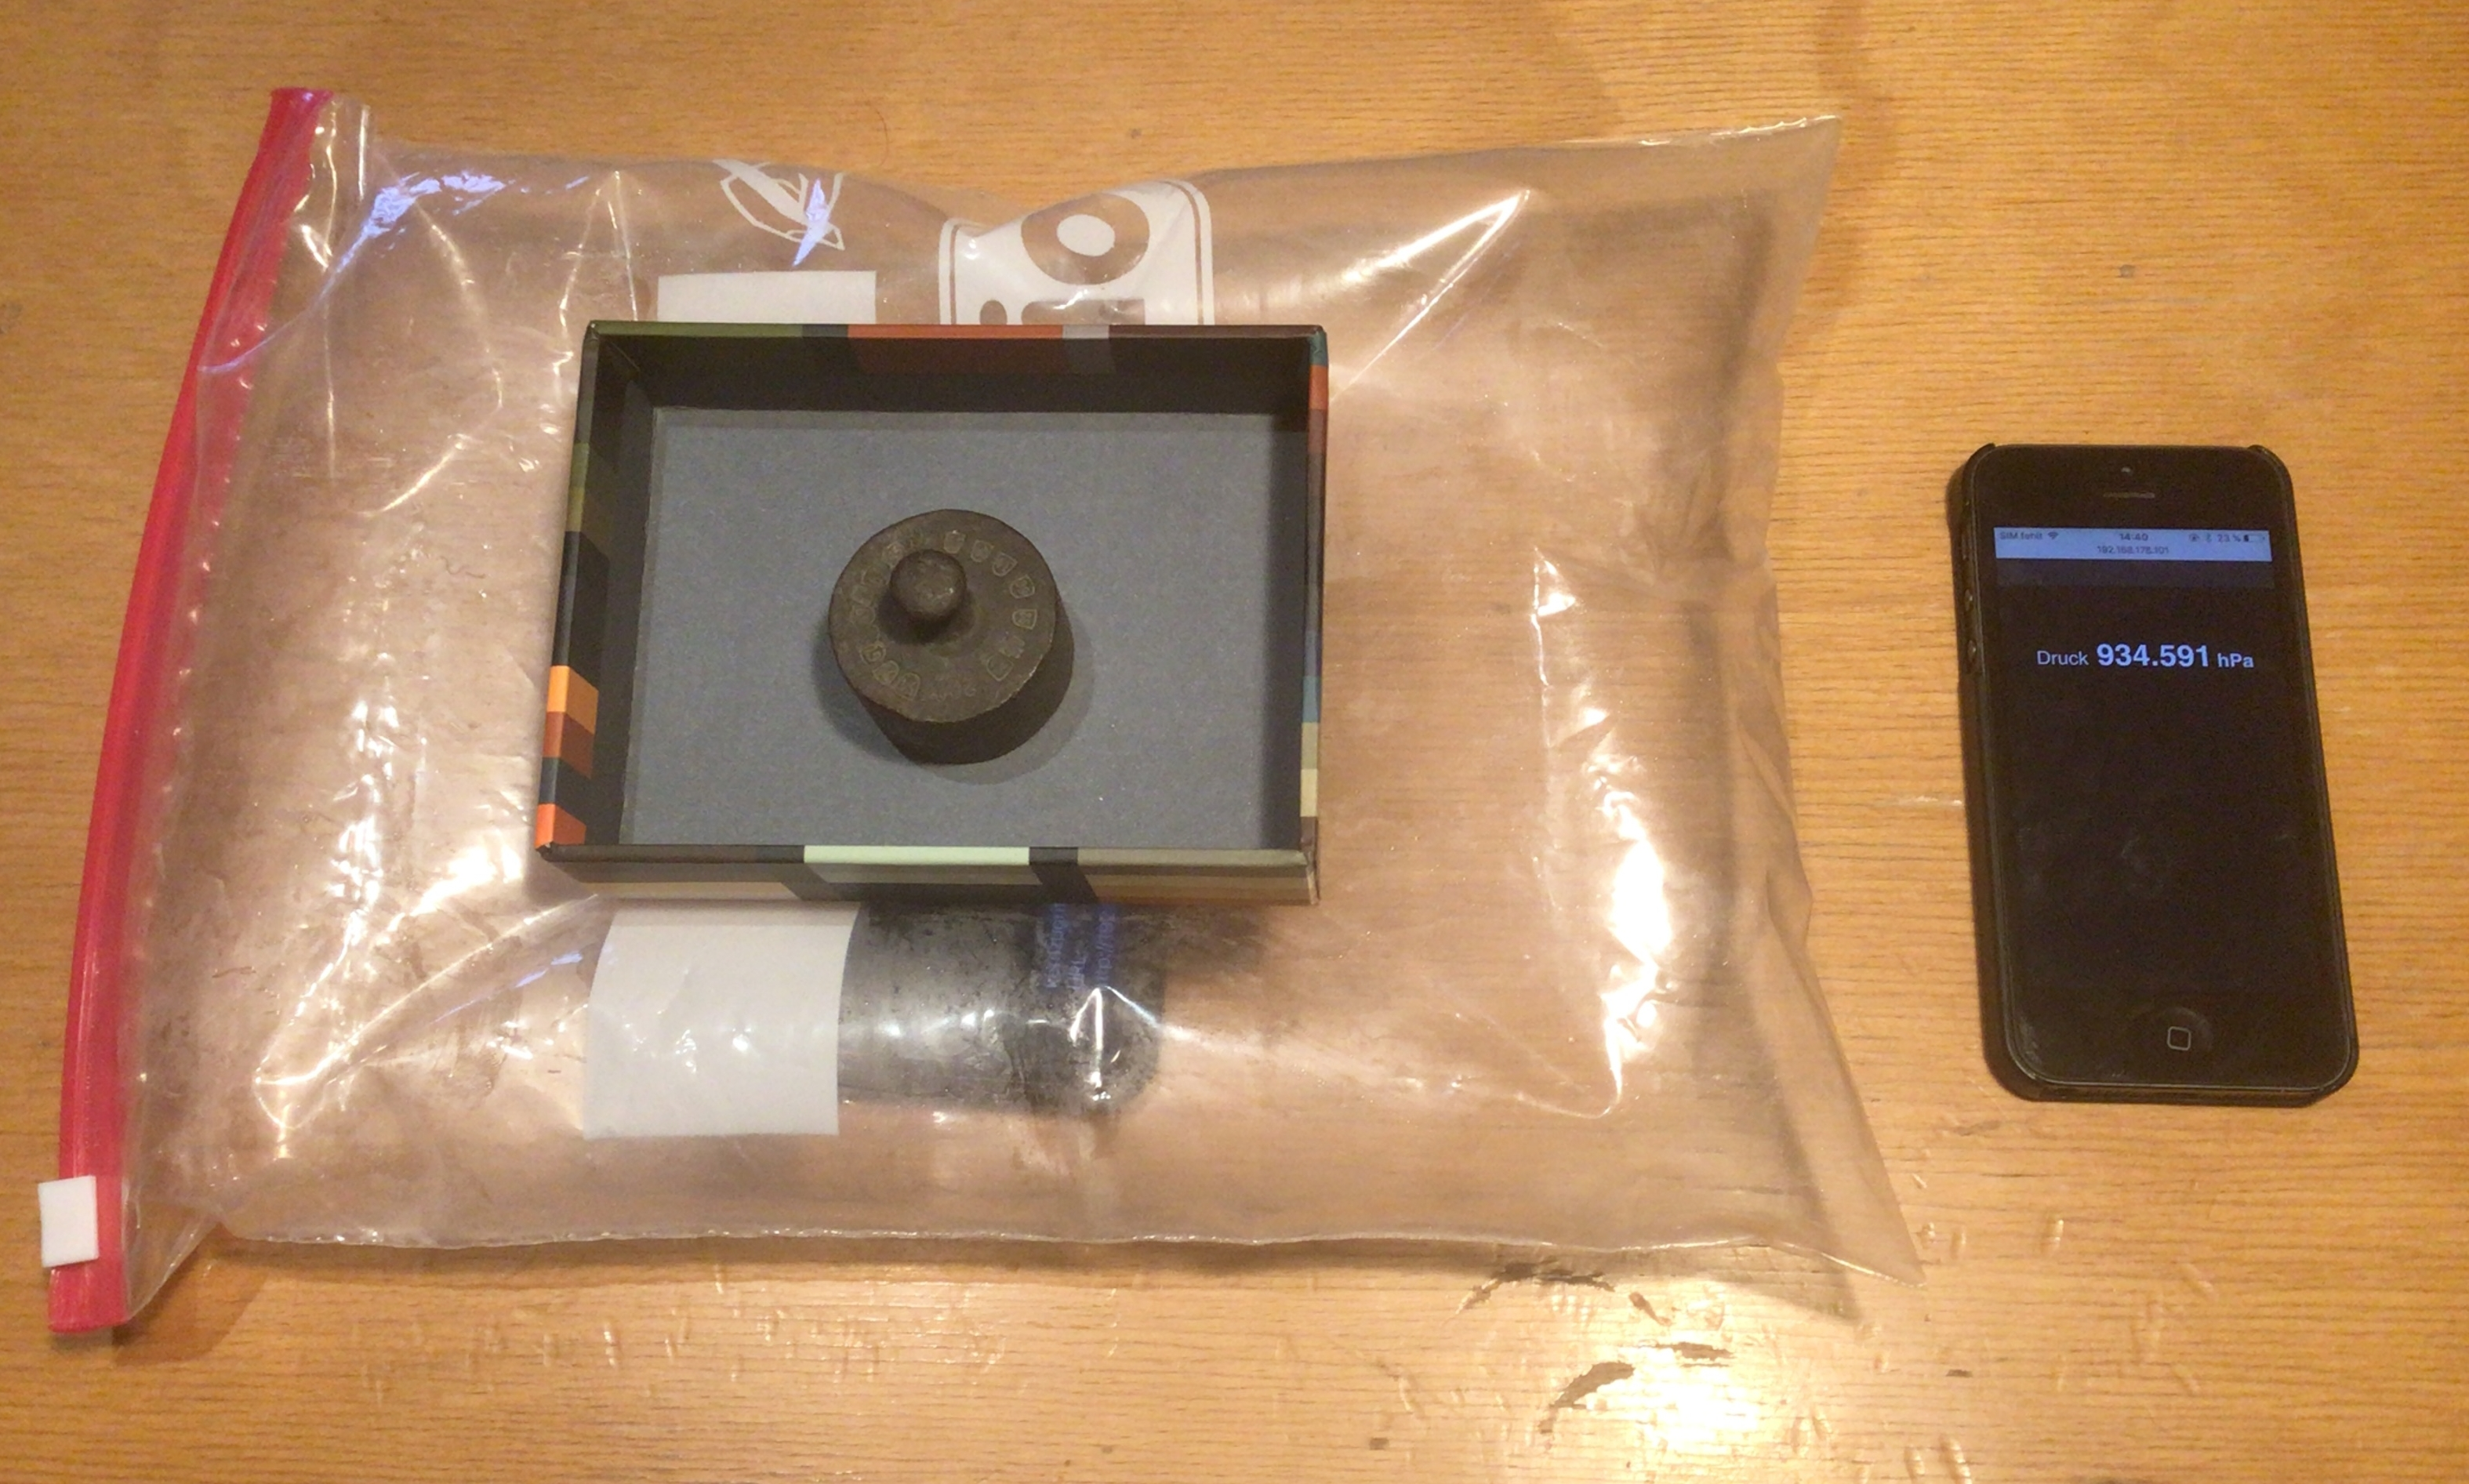
\includegraphics[width=0.85\textwidth]{img/versuchsaufbau}
    \end{minipage}
    \begin{minipage}[c]{0.5\textwidth}
        \begin{center}
            \begin{circuitikz} 
                \ctikzset{
                    bipoles/capacitor/width/.initial=.1,
                    european resistors
                }
                \draw   (0,0) node[spdt] (s) {}
                % middle part
                (s.in) to [short] (-1,0) coordinate (cr)
                (cr) to [C, l_={$C$}] (-2.5,0) coordinate (cl)
                (cl) to [short] (-5.5,0) coordinate (al)
                % bottom part             
                (al) to [short] (-5.5,-1.5) coordinate (al_down)
                (s.out 2) to [short] (s.out 2|-0,-1.5) coordinate (s_out_2_down)
                (al_down) to [short] (-4.1,-1.5) coordinate (motor_left)
                (motor_left) to [Telmech=M, name=M3] (s_out_2_down) 
                % top part
                (al) to [short] (-5.5,2) coordinate (al_up)
                (al_up) to [short] (-4.5,2) coordinate(bat_left)
                (s.out 1) to [short] (s.out 1|-0,2) coordinate (s_out_1_up)
                (s_out_1_up) to [short] (-2.5,2) coordinate (bat_right)
                (bat_right) to [battery1] (bat_left) 
                % voltage measurement
                (bat_right) to [short] (-2.5,1) coordinate (voltmeter_right)
                (bat_left) to [short] (-4.5,1) coordinate (voltmeter_left)
                (voltmeter_left) to [voltmeter] (voltmeter_right)
                ;
                \node at (-3,2.4) {$U$};
                \draw (al_down) ++ (0,0.3) node[ground]{}; 
            \end{circuitikz}
        \end{center}
    \end{minipage}

    \vspace{0.4cm}
    \textbf{Aufbau}: Das Experiment besteht aus einem Lade- und Entladestromkreis für den Kondensator. Ein Schalter ermöglicht den Wechsel. Für das Aufladen im Ladestromkreis wird ein Netzgerät verwendet. Zusätzlich wird ein Spannungsmessgerät für die besseren Darstellung der Ladespannung eingebaut. Im Entladestromkreis wird ein Elektromotor durch den Kondensator angetrieben. Durch diesen Motor wird ein Massestück, dass auf Höhe des Bodens hängt, angehoben. Gemessen wird die Höhe durch ein Höhenmaßstab mit Zeiger.   
    
    \vspace{0.4cm}
    \textbf{Durchführung}: Der Kondensator wird zunächst mit einer bestimmten Spannung aufgeladen. Anschließend wird im Entladestromkreis die Höhe gemessen, um die das Massestück vom Boden angehoben wird. Die Ladespannung wird in jedem Durchgang um $\Delta U=1$ V erhöht, bis $U=8$ V erreicht sind.

    \vspace{0.4cm}
    \textbf{Ergebnis}: Man beobachtet die Proportionalität
    \begin{align*}
        U^2 \sim h
    \end{align*}
    Für die Energie des aufgeladenen Kondensators $E_C$ und die potentielle Energie $E_{\text{pot}}$ des Massestücks gilt $E_{\text{C}} \sim E_{\text{pot}}=mgh$. Damit folgt $E_C \sim h$ und weiter
    \begin{align*}
        E_C \sim U^2
    \end{align*}
    
\vspace{0.4cm}
    \textbf{Didaktische Bemerkungen}: Durch Ändern der Kapazität des Kondensators bei konstanter Spannung lässt sich zusätzlich die Proportionalität $E_C \sim C$ zeigen. Damit erhält man insgesamt $E_C \sim CU^2$. Um das abschließende Ergebnis $E_K=\frac{1}{2}CU^2$ zu erhalten, müssen weiterführende Überlegungen angestellt werden. 

    \vspace{0.4cm}
    \textbf{Bemerkungen}: Die maximale Spannung von $U=8$ V sollte am Elektromotor nicht überschritten werden. 
\end{tcolorbox}
\end{document}
